% Exact LaTeX recreation of the supplied Phase-1.pdf
% Compile with pdfLaTeX. Place member pictures in the same folder if required.

\documentclass[11pt,a4paper]{article}

\usepackage[a4paper,left=2.0cm,right=2.0cm,top=1.55cm,bottom=1.55cm]{geometry}
\usepackage[T1]{fontenc}
\usepackage{lmodern}
\usepackage{graphicx}
\usepackage{xcolor}
\usepackage{array}
\usepackage{tabularx}
\usepackage{ragged2e}
\usepackage{enumitem}
\usepackage{fancyhdr}
\usepackage{tikz}
\usepackage{setspace}

% -------------------------------------------------
% COLOURS
% -------------------------------------------------
\definecolor{TitleBlue}{RGB}{61,103,154}

% -------------------------------------------------
% GENERAL SETTINGS
% -------------------------------------------------
\setlength{\parindent}{0pt}
\setlength{\parskip}{0pt}
\renewcommand{\arraystretch}{1.0}

% The supplied document uses a clean sans-serif heading style
% and italic serif-style explanatory text.
\newcommand{\blueheading}[1]{%
    {\sffamily\color{TitleBlue}\fontsize{15}{18}\selectfont #1}%
}

\newcommand{\bluebigheading}[1]{%
    {\sffamily\bfseries\color{TitleBlue}\fontsize{16}{19}\selectfont #1}%
}

\newcommand{\instruction}[1]{%
    {\itshape\fontsize{10.5}{12.5}\selectfont #1}%
}

\newcommand{\answerbox}[2][3.0cm]{%
    \vspace{2pt}
    \noindent
    \fbox{%
        \begin{minipage}[t][#1][t]{\dimexpr\textwidth-2\fboxsep-2\fboxrule\relax}
            \vspace{1mm}
            \itshape #2
        \end{minipage}
    }
}

% -------------------------------------------------
% HEADER / FOOTER
% -------------------------------------------------
\pagestyle{fancy}
\fancyhf{}
\renewcommand{\headrulewidth}{0pt}
\renewcommand{\footrulewidth}{0pt}

\fancyhead[L]{%
    \sffamily\bfseries\itshape\fontsize{10.5}{12}\selectfont
     B.Tech DSCPP-III-2026-T179 
}
\fancyhead[R]{%
    \sffamily\bfseries\fontsize{10.5}{12}\selectfont
    PROJECT PROPOSAL
}
\fancyfoot[R]{%
    \itshape\fontsize{10}{12}\selectfont
    Page \thepage
}
\setlength{\headheight}{14pt}
\setlength{\headsep}{23pt}
\setlength{\footskip}{24pt}

% -------------------------------------------------
% PAGE 1
% -------------------------------------------------
\begin{document}

\vspace*{4mm}

\bluebigheading{PROJECT AND TEAM INFORMATION}

\vspace{13mm}

\blueheading{Project Title}

\vspace{1mm}

\instruction{}

\answerbox[1.0cm]{Adaptive Traffic Signal System With Emergency Evacuation Support}

\vspace{13mm}

\blueheading{Student / Team Information}

\vspace{2mm}

% Team information table
% Compact 4-member layout so all members remain on Page 1.
\noindent
\begin{tabularx}{\textwidth}{|>{\RaggedRight\arraybackslash}p{0.69\textwidth}|>{\RaggedRight\arraybackslash}X|}
\hline
\begin{minipage}[t]{\linewidth}
\vspace{1.5mm}
\textit{Team Name:}\\[1mm]

\vspace{1.5mm}
\end{minipage}
&
\begin{minipage}[t]{\linewidth}
\vspace{1.5mm}
\textit{Four Bytes}
\vspace{1.5mm}
\end{minipage}
\\
\hline
\begin{minipage}[t][3.25cm][t]{\linewidth}
\vspace{1.5mm}
\textbf{Team member 1 (Team Lead)}\\[-1mm]

\vspace{2.0cm}
\end{minipage}
&
\begin{minipage}[t][3.25cm][t]{\linewidth}
\vspace{1.5mm}
\textit{Goyal, Riya - 2510013064}\\
\textit{2510013064@geu.ac.in}

\vspace{2mm}
\includegraphics[width=3.0cm,height=1.5cm,keepaspectratio]{member1.png}
\end{minipage}
\\
\hline
\begin{minipage}[t][3.25cm][t]{\linewidth}
\vspace{1.5mm}
\textbf{Team member 2}\\[-1mm]

\vspace{2.0cm}
\end{minipage}
&
\begin{minipage}[t][3.25cm][t]{\linewidth}
\vspace{1.5mm}
\textit{Smriti, Divya - 2510012531}\\
\textit{2510012531@geu.ac.in}

\vspace{2mm}
\includegraphics[width=3.0cm,height=1.5cm,keepaspectratio]{member2.png}
\end{minipage}
\\
\hline
\begin{minipage}[t][3.25cm][t]{\linewidth}
\vspace{1.5mm}
\textbf{Team member 3}\\[-1mm]

\vspace{2.0cm}
\end{minipage}
&
\begin{minipage}[t][3.25cm][t]{\linewidth}
\vspace{1.5mm}
\textit{Verma, Anushka - 2510380276}\\
\textit{2510380276@geu.ac.in}

\vspace{2mm}
\includegraphics[width=3.0cm,height=1.5cm,keepaspectratio]{member3.png}
\end{minipage}
\\
\hline
\begin{minipage}[t][3.25cm][t]{\linewidth}
\vspace{1.5mm}
\textbf{Team member 4}\\[-1mm]

\vspace{2.0cm}
\end{minipage}
&
\begin{minipage}[t][3.25cm][t]{\linewidth}
\vspace{1.5mm}
\textit{Soni, Tanishka - 2510380269}\\
\textit{2510380269@geu.ac.in}

\vspace{2mm}
 \includegraphics[width=3.0cm,height=1.5cm,keepaspectratio]{member4.png}
\end{minipage}
\\
\hline
\end{tabularx}

\newpage

% -------------------------------------------------
% PAGE 2
% -------------------------------------------------

\bluebigheading{PROPOSAL DESCRIPTION}

\vspace{12mm}

\blueheading{Motivation }

\vspace{1mm}

\instruction{}

\answerbox[10.0cm]{Unnecessary traffic delays are more than common in urban regions mainly in traffic intersections where, most of the time, traffic signals are having fixed timers.The most mentioned and relevant off all facts here is that these arrangements are: Failing to handle in an efficiently manner the dynamically shifting traffic situations, that directly leads to an extended waiting period for the drivers and a high density of traffic at those links.Making the matters even more complex and more often during the happening of a crises such as fires, accidents and medical crises. In such situation both the normal people and the authorities of emergency services depend on the fast and unharmed exit from the congested passages of the thoroughfare. Those who were missing would to be able to run away of the incident. Frontiers while ambulances. Same thing, the fire equipment would really desire a very quick access to the point of the fire.The aim of this project is designing and implementation of an Adaptive Traffic Signal System with the flexible system to support emergency evacuation. This can propose the traffic signal cycle as the current road load to range definition the transportation. The provisions, the present in shared with the professionalism- erams. It noted that the provisions can be is to give concern to While adversely influencing the capability of surviving roads by diverting traffic through irregularly routes which are more expected to be further exhausted and safer can alternatively facilitate emergency while diverting traffic through less exhausted and safer roads.The14 an adaptable approach of traffic dealing in combination with procedures for emergency evacuation Wants to attain these levels of benefits: enhanced transportation movement, decrees await period, and enhanced safety for pedestrians and other drivers, but for sure this undertaking can, and probably will, use article called object programming and info structure \& algorithms principles.}

\vspace{12mm}

\blueheading{State of the Art / Current solution }

\vspace{1mm}

\instruction{}

\answerbox[10.0cm]{Most of the traffic lights in current use are managed by fixed timings. In a no other vehicle (red yellow green) is in the visible range of field, the driving robot will receie its own proportional amount of green time, no matter the number of vehicles special for any vehicles waiting for the opportunity to cross.Too simple, it said, the fact is the idea of the each day's traffic circumstance is unpredictable so this kind of management could me always not only wasteful and irritating sometimes in - peak in which the cause of significant queue on road and time of waiting is the control signals of to the reason. In the efficient way of the meaning of humans and the reason, when the reasons for massive queue on road and wait the are fixed signals humans.These systems use sensors and cameras to measure the macrocosm and microcosm of the path of flow and than. override data collected. Which the signal timings are based on traffic class. Traffic solutions of this nature are Definitely goingto be benefits. Cost to implement may be high but the general flow of the traffics is smother more easierEmergency situations are normally. This traditional service is completely one system.For instance emergency supplying to ambulances and fire fighting. (see Figure 3.1.8 example of layout of trucks may be manual, traffic control or special traffic arrangement facilities.in this way, the evacuation. Calls for the cooperation of people in emergencies depends on the routes designed by the seconds, and instructions originating from those in charge.penalty, they may have situations in some of the doctors where use of those systems is designed to be forgiving as congested areas make roads unavailable.This projects make an instance, combining in what comes next way; traffic adaptive signal control with emergency evacuation support. Ourand evacuate the traffics more7.1The three.given very quickly.
}

\vspace{95mm}

\blueheading{Project Goals and Milestones }

\vspace{1mm}

\instruction{}

\answerbox[13.0cm]{PROJECT GOALS:

The advancement of an Adaptive Traffic Signal System for Emergency Evacuation is a goal of this project.Through which traffic management could be improved both on and emergency.The primary aspect of the system would be the ability to change the times of the traffic signals per traffic flow.And, the system could provide help over emergencies by providing emergency vehicles to the drivers which would be detected through the camera.Such as emergency cars and information guide with the route identification that is safe for evacuation.Another objective is to make use of Object-Oriented Programming and Data Structures which be applied to incorporate a kind of real-life image.Helped some out, the ideas in a practical for instance a scenario like roads vehicles junctions, signals are modeled as objects.Also, proper algorithms would be used to control which cars go and take the correct route.The main purpose of this project also the build of the Adaptive traffic signal system to support emergency evacuation is.Also the possibility to apply object oriented programming and data structures for the problem that is very current and practical.Besides modeling road networks vehicles junctions, traffic.To represent signal as objects, proper algorithms will be designed and implemented to handle the signal Traffic flow and path determination.

MILESTONES:

Milestone 1: Design the system level architecture, outline the key system class layouts Thecomponents.

Milestone 2: construction the simulation model of traffic signals and realization of normal operate of traffic traffic.

Milestone 3: Implement the adaptive signal control (by observing the density and level of..If: cost is difficult, then: congestion).

Milestone 4: Place together the emergency vehicle priority and the mechanisms for providing evacuate support.

Milestone 5: Run the system with different traffic simulations, measure performance and conclude all. Documents, presentations, and so on.}

\vspace{12mm}

\blueheading{Project Approach }

\vspace{1mm}

\instruction{}

\answerbox[8.5cm]{This project will be simulation of road system that relates roads junctions traffic signals and To create the mixture of different vehiclesit is based on implementation of programming by using C++ object-oriented programming (OOP) approachandComponents of Data StructuresMajor, classes depends on the understanding of the overall picture.1.7.I shall be to fact behind over view and approaches :Application of software modeling is to understanding of the interactions among (cars roads intersections, traffic lights which are the it is an essential step0.2.This road network will be modeled as a graph to represent Theconnections between locations. I would like to monitor the number of cars at each road intersection and in case of an event I will update the system to improve the management experience.To cope with emergency I have to designing the lights off time timer. System shall plan all possible routes allow the vehicles flow freely and synchronizing the signal light in case of emergency as to and the delay will be constant minimum between the different types a queues and priority queues (analyze the calculated between time betweenthere will be the basic unit.3.5.System will design the system to proceed in phases: starting from general traffic then to the adaptive signal control and then to emergency evacuation support other modules in a customizable manner..Different traffic situations are going to be simulated and analyzed to optimize and make the system as efficient as possible. this project is base on to simulation of traffic that will demonstrate that actually an adaptive system of traffic control can do the traffic run better and also in emergency situations.}

\newpage

% -------------------------------------------------
% PAGE 3
% -------------------------------------------------

\blueheading{System Architecture (High Level Diagram)}

\vspace{1mm}

\instruction{}

\instruction{}

\answerbox[9.0cm]{
\centering
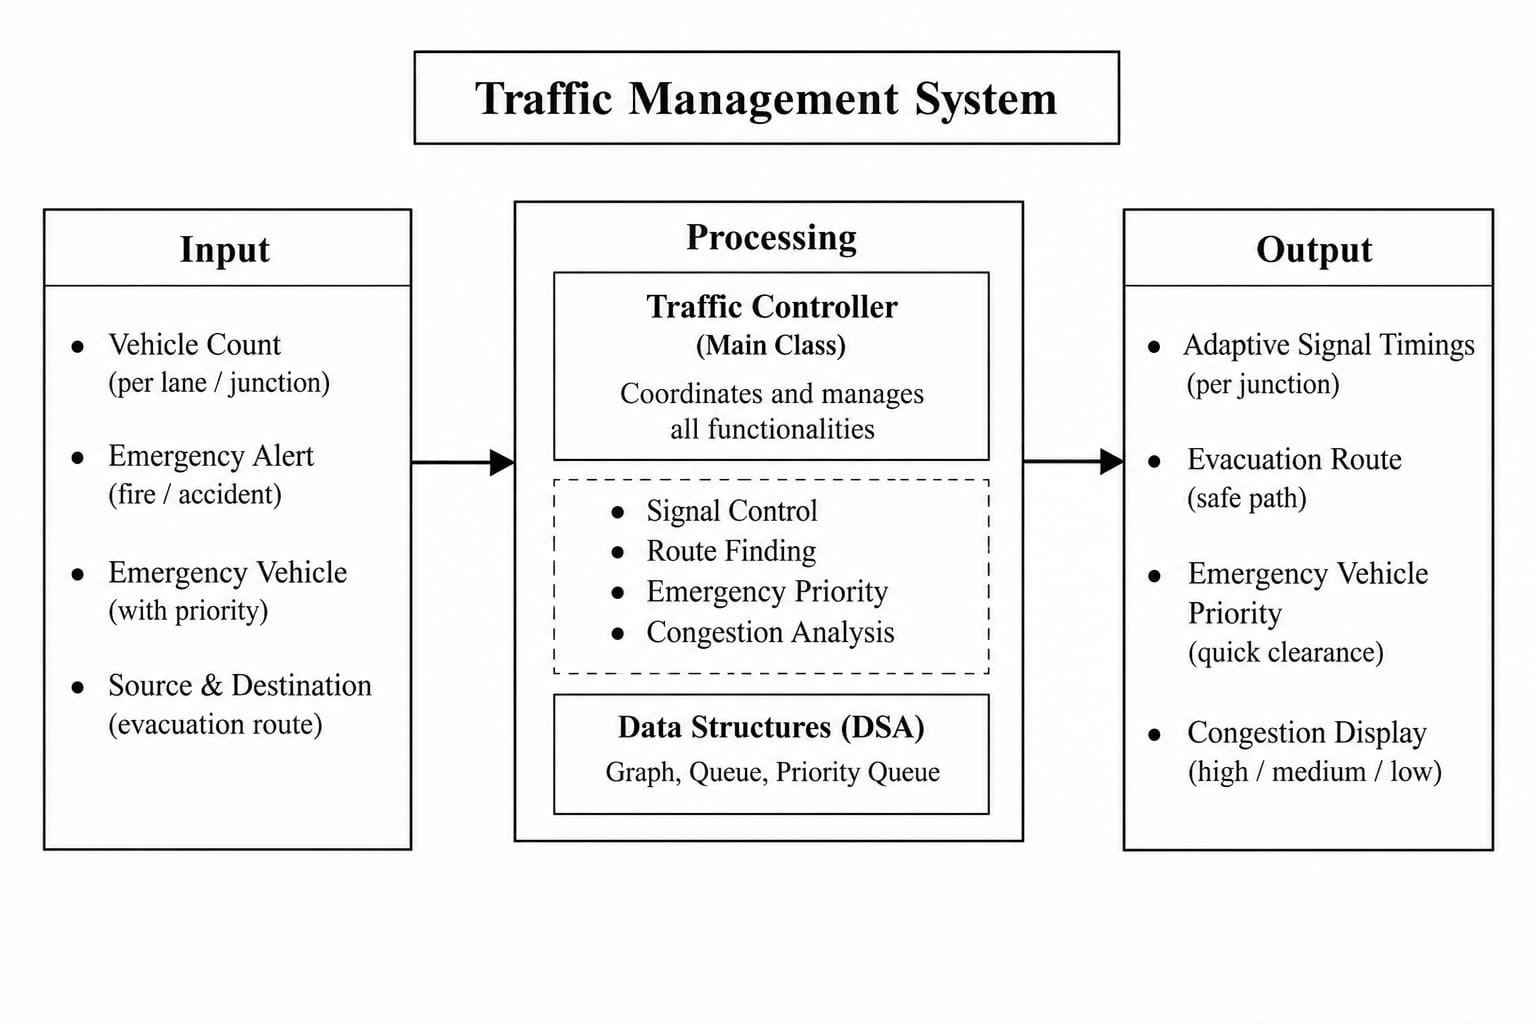
\includegraphics[width=0.9\linewidth,height=8cm,keepaspectratio]{diagram.jpeg}
}
\vspace{12mm}

\blueheading{Project Outcome / Deliverables }

\vspace{1mm}

\instruction{}

\answerbox[4.0cm]{Through a digital traffic management system, the main objective of this project is a streamlined process mainly for emergency situations. The system has the ability to set traffic signal lights by vehicle count at the intersection of streets.If an emergency, it directs emergency vehicles to reach the area first as a priority route is found. Besides this, the project explains OOPS with C++ and the application of data structures and algorithms concepts like graphs queues, priority queues and Dijkstra's algorithm. We expect to create a simple model depicting traffic levels, signal timing, first priority for emergency vehicles and the route chosen.}

\vspace{12mm}

\blueheading{Assumptions}

\vspace{6mm}

\instruction{}

\answerbox[5.0cm]{The project is focused on road network of small size having 4 to 8 junctions interlinked. The expert opinion says that, with this knowledge, traffic light timings can be adjusted based on the number of cars waiting in line at each junction. A safe zone and a hospital have been added as road layout of the project to cope up with the scenario of emergency. The road netwill be a graph representation. In this graph, the junctions are the nodes and roads are edges that
connect the nodes. The route-finding algorithms are the tools that can be applied to determine the most appropriate roads for emergency and evacuation vehicles and to avoid congestion.
It is also clear through this simulation-based research that we will not at all use the real data collected from vehicle GPS devices, traffic cameras, or sensors.}

\vspace{15mm}


\blueheading{References}

\vspace{1mm}

\instruction{}

\answerbox[2.0cm]{1.C++Reference—cppreference.com

2.Dijkstra’s Algorithm—CP-Algorithms

3.Class notes and reference materials provided by the faculty}

\end{document}
